

\section{Problema di interpolazione}
\dfn{}{
    Dati $n+1$ punti distinti $(x_0), (x_1,y_1), \dots, (x_n, y_n)$ con $x_0 < x_1 < \dots < x_n$ chiamati \textbf{nodi}, si definisce il \textbf{problema di interpolazione} quel problema che consiste nel trovare una funzione (polinomiale) $p(x)$ chiamata \textbf{interpolante}, tale che $\forall k \in [0,n],p(x_k) = y_k$
}

Esempietto con alcuni nodi:
\esempio{
    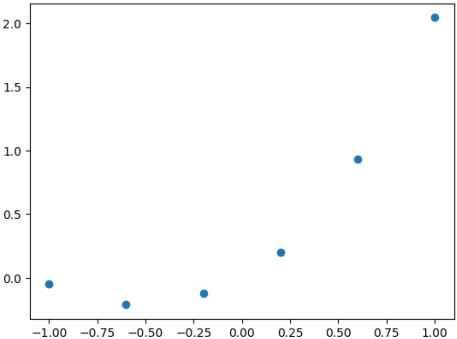
\includegraphics[width=10cm]{img/problema_interpolazione_esempio.png}
}

Si può risolvere il polinomio di grado $n$ come: 
\[
    p(x) = c_0 + c_1x + c_2x^2 + \dots + c_nx^n    
\]

Per identificare questo polinomio, ordunque, serve \red{calcolare i coefficienti} $c_i, i\in[1,n]$

\subsection{Esistenza dell'unicità}

\teorema{
    $\forall i\in[1,n], \forall (x_i, y_i)$ con $i$ nodi $t_i$, distinti tra loro, esiste un
    unico polinomio di grado minore od uguale a $n$, che indichiamo $P_n(x)$ con e chiamiamo
    polinomio interpolatore dei valori $y_i$ nei nodi $t_i$, tale che
    \[
        p_n(x_i) = y_i,i = 0,\dots, n    
    \]
}

Per la dimostrazione serve prima enunciare un lemma (che non verrà dimostrato)
\mlenma{}{
    Sia $r_n(x)$ un polinomio a coefficienti reali di grado $n$, il numero massimo di zeri distinti è $n$, ovvero:
    \begin{itemize}
        \item Un polinomio di grado $n$ può annullarsi in al massimo $n$ punti distinti.
        \item Se un polinomio di grado $n$ si annulla in più di $n$ punti distinti, allora deve essere il polinomio nullo, cioè identicamente uguale a zero per ogni valore di $x$
        
    \end{itemize}
}

\dimostrazione{
    Assumiamo che esistano due polinomi distinti di grado $n$, ovvero $p_n(x) \text{ e }q_n(x)$ che soddisfino entrambi le relazioni nodali precedenti. La loro differenza $p_n(x) - q_n(x)$ è ovvio verificare che è un polinomio di grado $n$ che si annulla in $n+1$ punti distinti. Per il fatto che il polinomio si annulla in $n+1$ punti e per il lemma enunciato si ha che $p_n(x) - q_n(x) = 0$, quindi $p_n(x) = q_n(x)$. Per assurdo dimostrato

    Q.e.d
}

\subsection{Calcolo del polinomio di interpolazione}

\subsubsection{Metodo classico}
È ovvio verificare che i coefficienti del polinomio di interpolazione di $n+1$ punti $(x_i, y_i)=(x_i, f(x_i))$ si potrebbero calcolare risolvendo il sistema lineare:
\[
    \begin{cases}
        c_0 + c_1x_1 + \dots + c_n x^n_1 = y_1 \\
        c_0 + c_1x_2 + \dots + c_n x^n_2 = y_2 \\
        \cdots \\
        c_0 + c_1x_n + \dots + c_n x^n_n = y_n
    \end{cases}
\]
Tuttavia la matrice dei coefficienti di questo sistema, detta \textbf{matrice di Vandermonde} può essere molto mal condizionata. Inoltre la risoluzione del sistema lineare richiede almeno $O(\frac{n^3}{3})$

\subsubsection{Metodo del polinomio interpolatore di Lagrange}

Introduciamo i polinomi base di lagrange
\dfn{}{
    Si chiamano \textbf{polinomi base di Lagrange} di grado $n$ particolari funzioni tali che:
    \[
        \phi_k(x_j) = \delta_{k,j}
    \]
    dove $k = j \implies \delta_{k,j}=1$ e $k \neq j \implies \delta_{k,j}=0$
}

La funzione $\phi_k(x)$ può essere scritta come:
\[
    \phi_k(x) = \prod_{j=0, j\neq k} ^ n \frac{x - x_j}{x_k - x_j}
\]
Si può notare, infatti, che include tutti i punti $x_j$ tranne $x_k$, quindi l'indice $j$ percorre tutti gli indici da $0$ a $n$ e nel caso in cui la $x$ in input sia diversa da $x_k$ vi sarà un $x_j$ tale che $x_j = x$, in quel caso il numeratore farà $0$ e renderà nulla la productoria. Nel caso, invece, la $x$ in input sia uguale a $x_k$ avremo $\frac{x_k - x_j}{x_k - x_j} \forall j$ rendendo la productoria uguale ad $1$.

Definito il polinomio posso scrivere il polinomio di interpolazione di Lagrange:
\dfn{}{
    Si chiama \textbf{polinomio interpolatore di Lagrange} tale funzione:
    \[
        p_n(x) = y_0\phi_0(x) + y_1\phi_1(x) + \dots + y_n\phi_n(x) = \sum_{k=0}^n y_k\phi_k(x)
    \]
}

Infatti soddisfa le condizioni di interpolazione
\[
    p_n(x_i)= \sum_{k=0}^n y_k\phi_k(x_i) = \sum_{k=0}^n y_k\delta_{i,k} = y_i
\]
\subsection{Errore di un polinomio interpolatore di una funzione}

Iniziamo con la definizione di un polinomio interpolatore di una funzione

\dfn{}{
    Sia $f[0,n] \to \mathbb{R}$ una funzione continua nel suo dominio e sia $y_i = f(x_i), \forall i \in [0,n]$. Sia anche $p_n(x)$ il polinomio interpolatore nei punti $(x_0, y_0), (x_1,y_1), \dots, (x_n, y_n)$

    Allora $p_n(x)$ è detto \textbf{polinomio interpolatore di $f$} e si denota:
    \[
        p_n(f)
    \]

}

Attraverso il polinomio di Lagrange è possibile quantificare l'errore che si commette sostituendo ad una funzione $f$ il suo polinomio interpolante attraverso il seguente teorema

\teorema{
    Sia $I$ un intervallo limitato, e si considerino $n + 1$ nodi di interpolazione distinti $x_i , i = 0, \dots , n$ in $I$. Sia $f$ derivabile con continuità fino all’ordine $n + 1$ in $I$. Allora
    \[
        \forall x \in I. \exists \eta  \in I: E(x) = f(x)- p_n(x) = \frac{f^{n+1(\eta)}}{(n+1)!} \prod_{i=0}^n (x - x_i)
    \] 

    E dove ovviamente $E(x_i) = 0$ dove $i=0,\dots n$
}

l'obbiettivo di questo teorema, quindi, è fornire una formula da cui ricavare un \textbf{errore di interpolazione} $E(x)$, che è la differenza tra la funzione originale $f(x)$ e il polinomio interpolante $p_n(x)$ nei punti in cui non conosciamo il valore esatto di $f(x)$ (ovvero tutti i punti diversi dai nodi)

Da questo \red{teorema non riusciamo a dedurre che}, qualsiasi sia la distribuzione dei
nodi, $max_{x\in I}|E(X)|\to 0$ per $n\to\infty$ ovvero (\red{che il massimo valore dell'errore} $E(x)=f(x)-p_n(x)$ su un intervallo $I$ \red{tende a zero al crescere di  $n$}). Esistono, infatti, alcune funzioni, come la funzione di
Runge, in cui per determinate scelte dei nodi, per esempio equidistanti dove  $max_{x\in I}|E(X)|\to \infty$ per $n\to\infty$. Alla luce di questa considerazione si ha che ad un aumento del grado $n$ del polinomio interpolatore non corrisponde necessariamente un miglioramento nella ricostruzione di una funzione $f$.

\begin{figure}[h!]
    \centering
    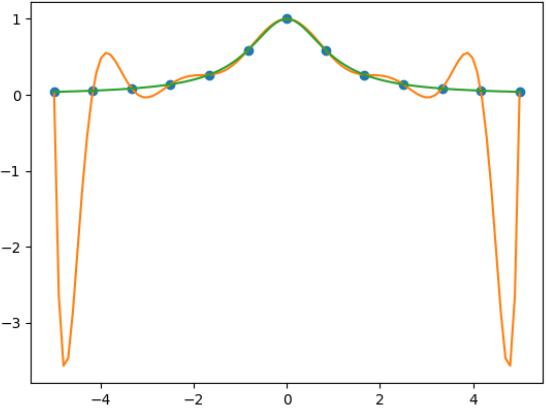
\includegraphics[width=8cm]{img/runge_interpolato_male.png}
    \caption{In questa immagine troviamo la funzione di Runge (in arancione) e il suo polinomio interpolante (in verde), dove la scelta dei nodi ha causato un errore di interpolazione elevato.}
    \label{fig:runge_interpolazione}
\end{figure}

Il fenomeno di Runge può essere evitato utilizzando opportune distribuzioni di nodi. In
particolare, su un arbitrario intervallo $[a, b]$ consideriamo i cosiddetti \textbf{nodi di Chebyshev-
Gauss-Lobatto}:
\[
    x_i = \frac{a+b}{2} - \frac{b-a}{2} \cos{(\frac{i\pi}{n})} \quad \text{con }i= 0 ,\dots, n   
\]

Notiamo che $x_i = \cos{(\frac{i\pi}{n})}$ se $[a,b] = [-1,1]$. Si può dimostrare che se $f$ è una funzione continua e derivabile con continuità in $[a,b]$ il polinomio interpolante $p_n(x)$ converge a $f(x)$ per $n\to\infty$

\begin{figure}[h!]
    \centering
    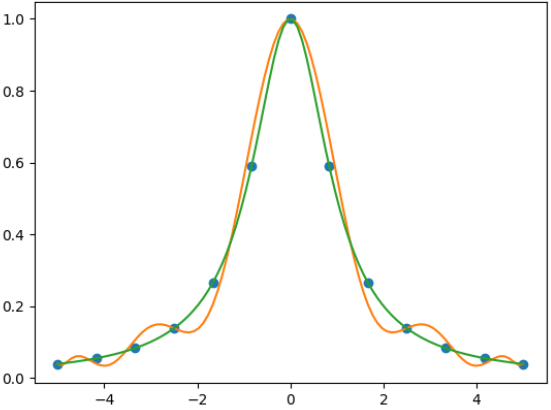
\includegraphics[width=8cm]{img/runge_interpolato_bene.png}
    \caption{in questa immagina la scelta dei nodi ha causato un errore di interpolazione relativamente basso}
    \label{fig:runge_interpolazione_bella}
\end{figure}

\subsection{Condizionamento dell’interpolazione polinomiale}

Alle volte non si dispone della funzione $f(x_i)$ relativi ai nodi $x_i$, con $i=0,\dots, n$ in un intervallo $I$ ma solo della sua approssimazione, denotata $\tilde{f}(x_i)$. La  perturbazione $f(x_i) - \tilde{f}(x_i)$ potrebbe essere dovuta ad esempio all'effetto degli errori di arrotondamento o ad errori di misura. Se chiamiamo $\tilde{p}_n{x}$ il polinomio interpolatore dei nodi $(x_i, \tilde{f}(x_i))$, si ha:
\[
    \max_{x\in I} |p_n(x) - \tilde{p}_n(x)| = \max_{x\in I}(\sum^n_{i=0}(f(x_i)-\tilde{f}(x_i)\phi_i(x))) =  \Lambda_n (x) \max |f(x_i) - \tilde{f}(x_i)|
\]

Dove $\Lambda_n (x)$ è il numero di condizione che in questo caso è:
\[
    \Lambda_n (x) = \max_{x\in I} |\sum_{i=0}^{n}\phi_i(x)|
\]
Che viene detta \textbf{costante i Lebesgue} che nel caso dell’interpolazione polinomiale su nodi equispaziati la costante di Lebesgue assume il valore:
\[
    \Lambda_n(x) \simeq \frac{2^{n+1}}{n(\log(n) + \gamma) e}    
\]
Dove $\gamma \simeq 5.47721$ è la \textbf{costante di Eulero}. Ciò comporta che per $n$ grande \red{questo tipo di interpolazione potrebbe essere instabile}
